\documentclass[aspectratio=169]{beamer}
\usetheme{simple}

\input{preamble/preamble.tex}
\input{preamble/preamble_math.tex}
% \input{preamble/preamble_acronyms.tex}

\title{Linear Gaussian Latent Variable Models}
\subtitle{STATS305B: Applied  Statistics II}
\author{Scott Linderman}
\date{\today}


\begin{document}


\maketitle

\begin{frame}{Last Time...}
    \begin{itemize}
        \item Mixture Models \& the EM Algorithm
        \item HMMs \& the Forward-Backward Algorithm
    \end{itemize}
\end{frame}

\begin{frame}{Today...}
    \textbf{Outline:}
    \begin{itemize}
        \item Principal Components Analysis (PCA)
        \item PCA as a linear Gaussian latent variable model
        \item Factor analysis
        \item Linear Dynamical Systems \& the Kalman Filter/Smoother
    \end{itemize}
    \vspace{1em}
\end{frame}

\begin{frame}[t]{Motivating Example}
    
Take HW3 as an example: you have temperature measurements at 9504 locations across the globe. Are the measurements really 9504 dimensional?

We might have a few objectives in mind:
\begin{itemize}
    \item \textbf{Dimensionality reduction:} are there a few dimensions along which the temperatures primarily vary? Maybe northern and southern hemisphere, or land and sea?
    
    \item \textbf{Visualization:} Sometimes, we want to embed high-dimensional points in 2 or 3 dimensions for visualization.
    
    \item \textbf{Compression:} How can I best summarize the data if I am willing to sacrifice some reconstruction accuracy?
\end{itemize}

\end{frame}

\begin{frame}{Principal Components of Global Temperature}
    \begin{figure}
        \centering
        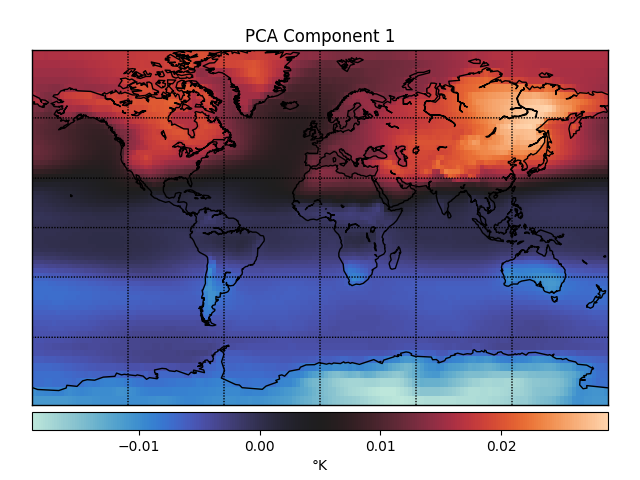
\includegraphics[width=0.7\textwidth]{12_lglvms/pc1.png}
        \caption{First PC of global temperature data.}
        \label{fig:pc1}
    \end{figure}
\end{frame}

\begin{frame}{Principal Components of Global Temperature}
    \begin{figure}
        \centering
        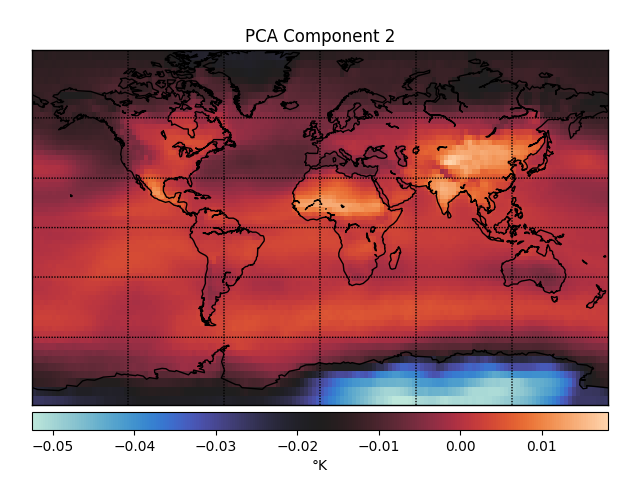
\includegraphics[width=0.7\textwidth]{12_lglvms/pc2.png}
        \caption{Second PC of global temperature data.}
        \label{fig:pc2}
    \end{figure}
\end{frame}

\begin{frame}{Principal Components of Global Temperature}
    \begin{figure}
        \centering
        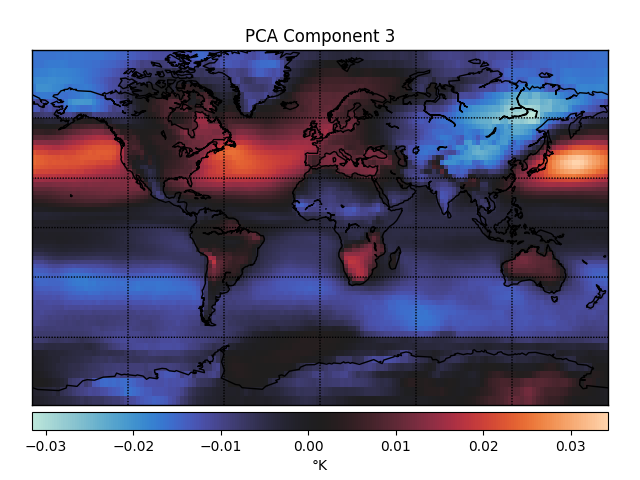
\includegraphics[width=0.7\textwidth]{12_lglvms/pc3.png}
        \caption{Second PC of global temperature data.}
        \label{fig:pc3}
    \end{figure}
\end{frame}
    

\begin{frame}[t]{Principal Components Analysis (PCA)}
Two classical definitions:
\begin{enumerate}
    \item An orthogonal projection of the data onto a lower dimensional linear space, known as the \textit{principal subspace}, such that the variance of the projected data is maximized (Hotelling, 1933).
    \item The linear projection that minimizes the average projection cost, defined as the mean squared distance between the data points and their projections (Pearson, 1901).
\end{enumerate}

(Quoted from Bishop, Ch 12)
\end{frame}

\section{PCA: Maximum Variance Formulation}

\begin{frame}[t]{PCA: Maximum Variance Formulation}

\textbf{Goal: } Project data $\{\mbx_n\}_{n=1}^N$ onto a lower dimensional space of dimension $M < D$ while maximizing the variance of the projected data.

\textbf{Illustration:}
\end{frame}

\begin{frame}[t]{PCA: Maximum Variance Formulation II}

To start, assume $M = 1$. The principal subspace is defined by a unit vector $\mbu_1 \in \reals^D$. This is called the first \textbf{principal component}.

Projecting a data point $\mbx_n$ onto this subspace amounts to taking an inner product, $\mbu_1^\top \mbx_n$. These is variously called the \textbf{scores}, \textbf{embeddings}, or \textbf{signals}. 
\end{frame}

\begin{frame}[t]{PCA: Maximum Variance Formulation III}
The mean of the projected data is,
\begin{align}
    \frac{1}{N} \sum_{n=1}^N \mbu_1^\top \mbx_n = \mbu_1^\top \left( \frac{1}{N} \sum_{n=1}^N \mbx_n \right) = \mbu_1^\top \bar{\mbx},
\end{align}
where $\bar{\mbx}$ is the sample mean.

The variance is 
\begin{align}
    \frac{1}{N} \sum_{n=1}^N \left[ \mbu_1^\top \mbx_n - \mbu_1^\top \bar{\mbx} \right]^2 
    &= \frac{1}{N} \sum_{n=1}^N \left[ \mbu_1^\top (\mbx_n - \bar{\mbx}) \right]^2 \\
    &=\frac{1}{N} \sum_{n=1}^N \mbu_1^\top (\mbx_n - \bar{\mbx}) (\mbx_n - \bar{\mbx})^\top \mbu_1 \\
    % &=\mbu_1^\top \left(\frac{1}{N} \sum_{n=1}^N (\mbx_n - \bar{\mbx}) (\mbx_n - \bar{\mbx})^\top \right) \mbu_1 \\
    &=\mbu_1^\top \mbS \mbu_1
\end{align}
where $\mbS = \frac{1}{N} \sum_{n=1}^N (\mbx_n - \bar{\mbx}) (\mbx_n - \bar{\mbx})^\top \in \reals^{D \times D}$ is the sample covariance matrix.
\end{frame}

\begin{frame}[t]{PCA: Maximum Variance Formulation IV}
Now maximize the projected variance wrt $\mbu_1$, 
\begin{align}
    \mbu_1 &= \argmax_{\mbu \in \bbS_{D}} \mbu^\top \mbS \mbu.
\end{align}
This is the variational definition of the eigenvector with maximal eigenvalue! 

I.e., $\mbu_1$ is the eigenvector of $\mbS$ with the largest eigenvalue, $\lambda_1$.

% Taking the gradient wrt $\mbu_1$ and setting to zero,
% \begin{align}
%     \nabla \cL(\mbu_1) &= 2\mbS \mbu_1 - 2\lambda_1 \mbu_1 = 0 \Rightarrow \mbS \mbu_1 = \lambda_1 \mbu_1.
% \end{align}
% So $\mbu_1$ must be an eigenvector of $\mbS$.
% Left multiplying by $\mbu^\top$,
% \begin{align}
%     \mbu_1^\top \mbS \mbu_1 = \lambda_1,
% \end{align}
% so the projected variance $\mbu_1^\top \mbS \mbu_1$ is maximized when we choose $\mbu_1$ to be the eigenvector with the largest eigenvalue $\lambda_1$.


More generally, to find an $M$ dimensional principal subspace, take the $M$ eigenvectors $\mbu_1, \ldots, \mbu_M$ with the largest eigenvalues $\lambda_1, \ldots, \lambda_M$.

Since $\mbS$ is real and symmetric positive definite, the eigenvectors are orthogonal.

\end{frame} 

% \section{PCA: Linear Autoencoder Formulation}

% \begin{frame}[t]{PCA: Linear Autoencoder Formulation}
%     Now consider Pearson's formulation of PCA as the linear projection that minimizes the average projection cost, defined as the mean squared distance between the data points and their projections.
    
%     \textbf{Illustration:}
% \end{frame}

% \begin{frame}[t]{PCA: Linear Autoencoder Formulation II}
%     To formalize this, let
%     \begin{align}
%         \mbW = 
%         \begin{bmatrix}
%         | & & | \\
%         \mbw_1 & \cdots & \mbw_M \\
%         | & & |
%         \end{bmatrix} \in \reals^{D \times M} \quad \text{with} \quad \mbW^\top \mbW = \mbI
%     \end{align}
%     be an orthogonal basis for the principal subspace. 
    
%     We will \textbf{encode} each data point by subtracting the mean and projecting onto the principal subspace to obtain $\mbz_n = \mbW^\top (\mbx_n - \bar{\mbx})$. 
    
%     Since $\mbW$ is an orthogonal matrix, all we need to do to \textbf{decode} the encoded data point is multiply $\mbW \mbz_n$ and add back the mean. That gives us, 
%     \begin{align}
%         \hat{\mbx}_n = \mbW \mbz_n + \bar{\mbx} = \mbW \mbW^\top (\mbx_n - \bar{\mbx}) + \bar{\mbx}.
%     \end{align}
% \end{frame}

% \begin{frame}[t]{PCA: Linear Autoencoder Formulation III}
%     \textbf{Goal:} Find an orthogonal matrix $\mbW$ that minimizes the mean squared reconstruction error,
%     \begin{align}
%         \cL(\mbW) &= \frac{1}{N} \sum_{n=1}^N \|\mbx_n - \hat{\mbx}_n\|_2^2
%     \end{align}
%     We can write this in matrix notation instead. Let $\mbX \in \reals^{N \times D}$ be the \textbf{centered data matrix} with rows~$(\mbx_n - \bar{\mbx})^\top$.
%     Then,
%     \begin{align}
%         \cL(\mbW) 
%         &= \frac{1}{N} \Tr[(\mbX - \hat{\mbX})^\top (\mbX - \hat{\mbX})] \\
%         &= \frac{1}{N} \Tr[(\mbX - \mbX \mbW \mbW^\top)^\top (\mbX - \mbX \mbW \mbW^\top)] \\
%         &= \frac{1}{N} \Tr[(\mbX(\mbI - \mbW \mbW^\top))^\top (\mbX (\mbI - \mbW \mbW^\top))]\\
%         % &= \frac{1}{N} \Tr[(\mbI - \mbW \mbW^\top)^\top \mbX^\top \mbX (\mbI - \mbW \mbW^\top)] \\
%         &= \Tr[(\mbI - \mbW \mbW^\top)^\top \mbS (\mbI - \mbW \mbW^\top)]
%     \end{align}
%     where $\mbS = \frac{1}{N} \mbX^\top \mbX$ is the sample covariance matrix.
% \end{frame}

% \begin{frame}[t]{PCA: Linear Autoencoder Formulation IV}
%     Now apply the circular trace property,
%     \begin{align}
%         \cL(\mbW) 
%         &= \Tr[\mbS (\mbI - \mbW \mbW^\top) (\mbI - \mbW \mbW^\top)^\top]
%     \end{align}
%     \textbf{Question:} What does $(\mbI - \mbW \mbW^\top) (\mbI - \mbW \mbW^\top)^\top$ equal?
%     \mode<handout>{
%     Note that $\mbI - \mbW \mbW^\top$ is a projection matrix, and applying the projection operator twice doesn't change the result. Mathematically,
%     \begin{align}
%         (\mbI - \mbW \mbW^\top) (\mbI - \mbW \mbW^\top)^\top 
%         = \mbI - 2 \mbW \mbW^\top + \mbW \mbW^\top \mbW \mbW^\top
%         = \mbI - \mbW \mbW^\top
%     \end{align}
%     }
% \end{frame}

% \begin{frame}[t]{PCA: Linear Autoencoder Formulation V}
%     Thus, the objective simplifies to,
%     \begin{align}
%         \cL(\mbW) 
%         = \Tr[\mbS(\mbI - \mbW \mbW^\top)]
%         = \Tr[\mbS] - \Tr[\mbS \mbW \mbW^\top]
%         = \mathrm{const} - \Tr[\mbW^\top \mbS \mbW].
%     \end{align}
%     Let $\mbU \mbLambda \mbU^\top$ be the eigendecomposition of $\mbS$. (Since it is a covariance matrix, the eigenvectors are orthogonal.) 
%     Plugging in,
%     \begin{align}
%         \cL(\mbW) 
%         &= \mathrm{const} - \Tr[\mbW^\top \mbU \mbLambda \mbU^\top \mbW] \\
%         &= \mathrm{const} - \Tr\left[\mbW^\top \left( \sum_{d=1}^D \lambda_d \mbu_d \mbu_d^\top \right) \mbW\right] \\
%         &= \mathrm{const} - \sum_{m=1}^M \sum_{d=1}^D \lambda_d \mbw_m^\top \mbu_d \mbu_d^\top \mbw_m \\
%         &= \mathrm{const} - \sum_{m=1}^M \sum_{d=1}^D \lambda_d (\mbw_m^\top \mbu_d)^2
%     \end{align}
%     \textbf{Question: } We want to minimize $\cL(\mbW)$ subject to $\mbW$ being orthogonal. What is the solution?
% \end{frame}

\begin{frame}[t]{PCA and the Singular Value Decomposition}
The first $M$ \textbf{principal components} are the leading $M$ \textbf{eigenvectors of the covariance matrix}. Equivalently, they are the first $M$ \textbf{right singular vectors of the data matrix}.

Let
\begin{align}
    \mbY = \frac{1}{\sqrt{N}} \mbX = \frac{1}{\sqrt{N}} \begin{bmatrix}
    - & (\mbx_1 - \bar{\mbx})^\top & - \\
    & \vdots & \\
    - & (\mbx_N^\top  - \bar{\mbx})^\top & -
    \end{bmatrix}
\end{align}
be the \textbf{centered and scaled} data matrix. Then $\mbY^\top \mbY = \frac{1}{N} \mbX^\top \mbX = \mbS$ is the covariance matrix.

The \textbf{singular value decomposition (SVD)} of $\mbY$ is,
\begin{align}
    \mbY = \mbV \mbLambda^{\frac{1}{2}} \mbU^\top 
    \Rightarrow \mbY^\top \mbY = \frac{1}{N} \mbU \mbLambda^{\frac{1}{2}} \mbV^\top \mbV \mbLambda^{\frac{1}{2}} \mbU^\top 
    = \frac{1}{N} \mbU \mbLambda \mbU^\top
\end{align}
I.e. the \textbf{right singular vectors} of $\mbY$ are the same (up to sign flips) as the eigenvectors of $\mbS$, and \textbf{singular values} of $\mbY$ are the square root of the eigenvalues of $\mbS$.
\end{frame}

\begin{frame}[t]{PCA Explained Variance}
How well do the $M$ principal components explain the data? 

Let $\mbz_n = \mbU_M^\top (\mbx_n - \bar{\mbx}) \in \reals^M$. Its covariance is,
\begin{align}
    \mathrm{Cov}[\mbz] = \mathrm{Cov}[\mbU_M^\top (\mbx - \bar{\mbx})] = \mbU_M^\top \mathrm{Cov}[\mbx] \mbU_M = \diag([\lambda_1, \ldots, \lambda_M]).
\end{align}

Of course, if we let $M = D$, then we have $\mathrm{Cov}(\mbz) = \diag([\lambda_1, \ldots, \lambda_D])$. 

One way of assessing how well $M$ components fits the data is via the \textbf{fraction of variance explained},
\begin{align}
    \text{variance explained} = \frac{\Tr(\mathrm{Cov}[z; M \text{ components}])}{\Tr(\mathrm{Cov}[z; D \text{ components}])} = \frac{\sum_{m=1}^M \lambda_m}{\sum_{m=1}^D \lambda_m} \in [0, 1].
\end{align}
\end{frame}

\begin{frame}{Scree Plots}
\begin{figure}
    \centering
    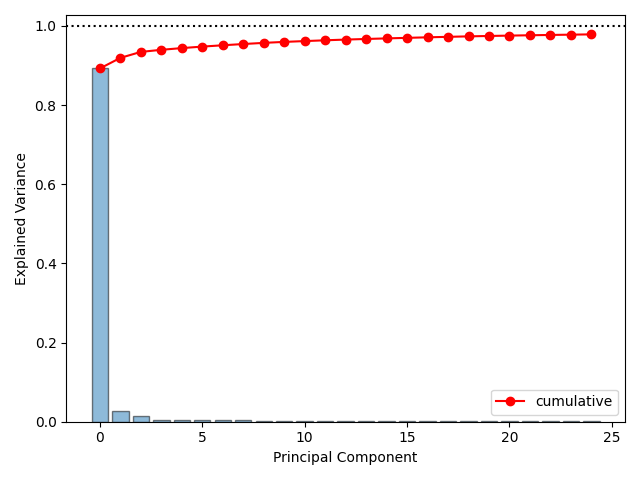
\includegraphics[width=0.7\textwidth]{12_lglvms/scree.png}
    \caption{``Scree'' plot showing percent variance explained per component and cumulatively.}
    \label{fig:scree}
\end{figure}
\end{frame}


\begin{frame}{Outline}
    \begin{itemize}
        \item Principal Components Analysis (PCA)
        \item \textbf{PCA as a linear Gaussian latent variable model}
        \item Factor analysis
        \item Linear Dynamical Systems \& the Kalman Filter/Smoother
    \end{itemize}
    \vspace{1em}
\end{frame}

\begin{frame}[t]{Probabilistic PCA: A Continuous Latent Variable Model}
    We cast the principal components as the solutions to an optimization problem: maximize the projected variance.
    
    A more modern view of PCA is as the \textbf{maximum likelihood estimate} of a \textbf{latent variable model}.
    
    \textbf{Probabilistic PCA} (PPCA) has many advantages:
    \begin{itemize}
        \item It's a multivariate normal model with \textbf{low-rank plus diagonal covariance}, which takes only $O(MD)$ parameters.
        \item We can fit the model using a \textbf{host of inference algorithms}, including EM.
        \item It can handle \textbf{missing data}.
        \item We can obtain posterior distributions of the principal components and scores. 
        \item It can be embedded in larger probabilistic models.
    \end{itemize}
\end{frame}

\begin{frame}[t]{Probabilistic PCA: A Continuous Latent Variable Model}
    The PPCA model is quite simple,
    \begin{align}
        \mbz_n &\iid{\sim} \cN(\mbzero, \mbI) \\
        \mbx_n \mid \mbz_n &\sim \cN(\mbW \mbz + \mbmu, \sigma^2 \mbI),
    \end{align}
    where $\mbz_n \in \reals^M$ is a latent variable, $\mbW \in \reals^{D \times M}$ are the weights, $\mbmu \in \reals^D$ is the bias parameter, and $\sigma^2 \in \reals_+$ is a variance. 
    
    Equivalently, we can think of $\mbx_n$ as a linear function of $\mbz_n$ with additive noise,
    \begin{align}
        \mbx_n &= \mbW \mbz_n + \mbmu + \mbepsilon_n,
    \end{align}
    where $\mbepsilon_n \sim \cN(\mbzero, \sigma^2 \mbI) \in \reals^D$.
\end{frame}

\begin{frame}[t]{Maximum likelihood estimation of the parameters}
    Suppose we only need a \textbf{point estimate} of the parameters $\mbW$, $\mbmu$, and $\sigma^2$. 
    
    A natural approach is the \textbf{maximum likelihood estimate} (MLE), 
    \begin{align}
        \mbW_{\mathsf{ML}}, \mbmu_{\mathsf{ML}}, \sigma^2_{\mathsf{ML}} = \argmax \cL(\mbW, \mbmu, \sigma^2),
    \end{align}
    where $\cL$ is the marginal likelihood,
    \begin{align}
        \cL(\mbW, \mbmu, \sigma^2) &= \log p(\mbX \mid \mbW, \mbmu, \sigma^2) \\
        &= \log \int \prod_{n=1}^N p(\mbx_n \mid \mbz_n, \mbW, \mbmu, \sigma^2) \, p(\mbz_n) \dif \mbz_n \\
        &= \log \int \prod_{n=1}^N \cN(\mbx_n \mid \mbW \mbz_n + \mbmu, \sigma^2 \mbI) \, \cN(\mbz_n \mid \mbzero, \mbI) \dif \mbz_n 
        % \\
        % &= \sum_{n=1}^N \log \cN(\mbx_n \mid \mbmu, \mbW \mbW^\top + \sigma^2 \mbI) 
    \end{align}
    \textbf{Exercise: } Simplify this expression.
\end{frame}

\begin{frame}[t]{Maximum likelihood estimation of the parameters II}
    The log likelihood simplifies to,
    \begin{align}
        \cL(\mbW, \mbmu, \sigma^2) 
        -\frac{ND}{2} \log 2 \pi - \frac{N}{2} \log |\mbC| -\frac{1}{2} \sum_{n=1}^N (\mbx_n - \mbmu)^\top \mbC^{-1} (\mbx - \mbmu) 
    \end{align}
    where $\mbC = \mbW \mbW^\top + \sigma^2 \mbI$. 
    
    Setting the derivative wrt $\mbmu$ to zero and solving yields $\mbmu_{\mathsf{ML}} = \bar{\mbx}$, the sample mean.
    
    Maximizing wrt $\mbW$ and $\sigma^2$ is more complex but still has a closed form solution,
    \begin{align}
        \mbW_{\mathsf{ML}} = \mbU_M (\mbLambda_M - \sigma^2 \mbI)^{\frac{1}{2}} \mbR,
    \end{align}
    where $\mbU_M \in \reals^{D \times M}$ has columns given by the leading eigenvectors of the sample covariance matrix $\mbS$, where $\mbLambda_M = \diag([\lambda_1, \ldots, \lambda_M])$, and where $\mbR \in \reals^{M \times M}$ is an arbitrary \textit{orthogonal} matrix.
    
    Put differently, the MLE weights are only identifiable up to orthogonal transformation. Or, only the subspace spanned by $\mbU_M$ is identifiable.
\end{frame}

\begin{frame}[t]{Maximum likelihood estimation of the parameters III}
    Finally, the MLE of the variance is,
    \begin{align}
        \sigma^2_{\mathsf{ML}} &= \frac{1}{D - M} \sum_{m=M+1}^D \lambda_m, 
    \end{align}
    the average variance in the remaining dimensions. 
    
    \textbf{Question: } What is the marginal covariance $\mbC$ using the MLE $\mbW_{\mathsf{ML}}$ and $\sigma^2_{\mathsf{ML}}$?
    
    \textbf{Question: } Intuitively, why is the marginal covariance invariant to rotations of the weights?
\end{frame}

\begin{frame}[t]{The Posterior Distribution on the Latent Variables}
    Now fix $\mbW$, $\mbmu$, and $\sigma^2$ (e.g. to their maximum likelihood values). What is the posterior of~$\mbz_n$?
    \begin{align}
        p(\mbz_n \mid \mbx_n, \mbW, \mbmu, \sigma^2) 
        &\propto \cN(\mbz_n \mid \mbzero, \mbI) \, \cN(\mbx_n \mid \mbW \mbz_n + \mbmu, \sigma^2 \mbI) \\
        &\propto \exp \left\{ -\frac{1}{2} \mbz_n^\top \mbz_n -\frac{1}{2} (\mbx_n - \mbW \mbz_n - \mbmu)^\top (\sigma^2 \mbI)^{-1} (\mbx_n - \mbW \mbz_n - \mbmu) \right\} \\
        &\propto \exp \left\{ -\frac{1}{2} \mbz_n^\top \mbJ_n \mbz_n + \mbh_n^\top\mbz_n \right\} \\
    \end{align}
    where $\mbJ_n = \mbI + \frac{1}{\sigma^2} \mbW^\top \mbW$ and $ \mbh_n = \frac{1}{\sigma^2} \mbW^\top (\mbx_n - \mbmu)$
    
    Completing the square,
    \begin{align}
        p(\mbz_n \mid \mbx_n, \mbW, \mbmu, \sigma^2) &= \cN(\mbz_n \mid \mbJ_n^{-1} \mbh_n, \mbJ_n^{-1}).
    \end{align}
    
    
\end{frame}

% \begin{frame}[t]{The Posterior Distribution on the Latent Variables II}
%     \textbf{Note:} You can compute $\mbJ_n^{-1}$ using the Woodbury matrix identity:
%     \begin{align}
%         \mbJ_n^{-1} &= (\mbI + \sigma^{-2} \mbW^\top \mbW)^{-1} \\
%         &= \sigma^2 ( \sigma^2 \mbI + \mbW^\top \mbW)^{-1} \\
%         &= \sigma^2 \left[ \sigma^{-2} \mbI - \sigma^{-2} \mbW^\top (\mbI + \sigma^{-2} \mbW \mbW^\top)^{-1} \mbW \sigma^{-2}  \right] \\
%         &= \mbI - \sigma^{-2} \mbW^\top (\mbI + \sigma^{-2} \mbW \mbW^\top)^{-1} \mbW 
%     \end{align}
% \end{frame}

\begin{frame}[t]{The Posterior Distribution in the Zero Noise Limit}
    In the limit where $\sigma^2 \to 0$, the posterior mean of $\mbz_n$ is,
    \begin{align}
        \lim_{\sigma^2 \to 0} \E[\mbz_n \mid \mbx_n, \mbW, \mbmu, \sigma^2] 
        &= \lim_{\sigma^2 \to 0} (\mbI + \frac{1}{\sigma^2} \mbW^\top \mbW)^{-1} [\frac{1}{\sigma^2} \mbW^\top (\mbx_n - \mbmu)] \\
        &= \lim_{\sigma^2 \to 0} (\sigma^2 \mbI + \mbW^\top \mbW)^{-1} \mbW^\top (\mbx_n - \mbmu) \\
        &= (\mbW^\top \mbW)^{-1} \mbW^\top (\mbx_n - \mbmu)
    \end{align}
    Now suppose $\mbW = \mbW_{\mathsf{ML}} = \mbU_M (\mbLambda_M - \sigma^2 \mbI)^{\frac{1}{2}} \mbR$ and set $\mbR = \mbI$. This goes to $\mbW = \mbU_M \mbLambda_M^{\frac{1}{2}}$. Then, 
    \begin{align}
        \lim_{\sigma^2 \to 0} \E[\mbz_n \mid \mbx_n, \mbW, \mbmu, \sigma^2] 
        &= (\mbW^\top \mbW)^{-1} \mbW^\top (\mbx_n - \mbmu) \\
        &= \mbLambda_M^{-\frac{1}{2}} \mbU_M^\top (\mbx_n - \mbmu)
    \end{align}
    % This is the same as $\mbz_n$ from the linear autoencoder formulation, except here the $\mbz_n$'s are scaled by $\mbLambda^{-\frac{1}{2}}$ to be unit variance in all dimensions.
    
    % However, in this limit the model is degenerate ($\mbC$ has rank $M < D$). With $\sigma^2 > 0$, the posterior mean \textbf{shrinks} toward the origin
\end{frame}

% \begin{frame}[t]{A Slight Reformulation of Probabilistic PCA}
%     In my opinion, one frustrating feature of PPCA is that since the latent variables (aka scores) $\mbz_n$ are standard normal random variables under the prior, the principal components (columns of $\mbW_{\mathsf{ML}}$) have to be scaled by $\mbLambda_M^{\frac{1}{2}}$. 
    
%     This is in contrast to classical PCA, where the \textit{scores} are scaled and the \textit{principal components} are normalized. 
    
%     Therefore, I propose a slight modification to the model:
%     \begin{align}
%         \mbz_n &\iid{\sim} \cN(\mbzero, \mbLambda) \\
%         \mbx_n &\sim \cN(\mbW \mbz_n + \mbmu, \sigma^2 \mbI),
%     \end{align}
%     where $\mbLambda = \diag([\lambda_1, \ldots, \lambda_M])$.
    
%     This model is \textbf{overparameterized} since for any $(\mbLambda, \mbW)$ pair we can achieve the same marginal likelihood with $(\mbI, \mbW \mbLambda^{\frac{1}{2}})$.
    
%     However, this model is easier to put priors on, and it generalizes nicely, as we'll see soon.
% \end{frame}

\begin{frame}[t, allowframebreaks]{EM for Probabilistic PCA}
    The \textbf{E-step} is to compute the posterior $q(\mbz_n) = p(\mbz_n \mid \mbx_n; \mbtheta)$, where $\mbtheta = (\mbW, \mbmu, \sigma^2)$ are the current parameters. For simplicity, assume the data is centered so that $\mbmu^\star = 0$. 
    
    The \textbf{M-step} is to maximize the expected complete data log likelihood,
    \begin{align*}
        \cL(\mbtheta) 
        &= \sum_{n=1}^N \E_{q(\mbz_n)} \left[ \log p(\mbx_n \mid \mbz_n; \mbtheta)\right] \\
        &= \sum_{n=1}^N \E_{q(\mbz_n)} \left[ \log \cN(\mbx_n \mid \mbW \mbz_n, \sigma^2 \mbI) \right] \\
        &= \sum_{n=1}^N \E_{q(\mbz_n)} \left[ -\frac{D}{2} \log \sigma^2 -\frac{1}{2\sigma^2} (\mbx_n - \mbW \mbz_n)^\top (\mbx_n - \mbW \mbz_n)\right].
    \end{align*}
    As a function of $\mbW$, 
    \begin{align*}
        \cL(\mbW) 
        &= \sum_{n=1}^N \E_{q(\mbz_n)} \left[ -\frac{1}{2\sigma^2} \left \langle \mbW^\top \mbW, \mbz_n \mbz_n^\top \right \rangle + \frac{1}{\sigma^2} \left \langle \mbW, \mbx_n \mbz_n^\top \right \rangle \right] \\
        &= -\frac{1}{2\sigma^2} \left \langle \mbW^\top \mbW, \sum_{n=1}^N \E_{q(\mbz_n)} \left[ \mbz_n \mbz_n^\top \right] \right \rangle + \frac{1}{\sigma^2} \left \langle \mbW, \sum_{n=1}^N \E_{q(\mbz_n)} \left[ \mbx_n \mbz_n^\top \right] \right \rangle.
    \end{align*}
    where $\langle \mbA, \mbB \rangle = \Tr(\mbA^\top \mbB)$ is the Frobenius inner product for matrices $\mbA$ and $\mbB$.

    Taking derivatives wrt $\mbW$ and setting to zero yields,
    \begin{align*}
        \mbW^\star &= \left( \sum_{n=1}^N \E_{q(\mbz_n)} \left[ \mbx_n \mbz_n^\top \right] \right) \left( \sum_{n=1}^N \E_{q(\mbz_n)} \left[ \mbz_n \mbz_n^\top \right] \right)^{-1}.
    \end{align*}
    It depends on sums of expected sufficient statistics! 

    \textbf{Exercise:} Derive the expected sufficient statistics and the M-step update for $\sigma^2$.
\end{frame}

% \begin{frame}[t, allowframebreaks]{Gibbs Sampling for Probabilistic PCA}
%     For simplicity, assume the data is centered and fix $\mbmu = 0$. Now let's put a prior on the parameters,
%     \begin{align}
%         p(\mbW, \sigma^2) &= \chi^{-2}(\sigma^2 \mid \nu_0, \sigma_0^2) \, \prod_{d=1}^D \cN(\mbw_d \mid \mbzero, \tfrac{\sigma^2}{\kappa_0} \mbI),
%     \end{align}
%     where $\mbw_d \in \reals^M$ are the \textit{rows} of $\mbW$.
    
%     Under this prior, the complete conditional distribution of the parameters is,
%     \begin{align}
%         p(\mbw_d \mid \{\mbx_n, \mbz_n\}_{n=1}^N, \sigma^2, \kappa_0) 
%         &\propto \cN(\mbw_d \mid \mbzero, \tfrac{\sigma^2}{\kappa_0} \mbI) \prod_{n=1}^N \cN(x_{n,d} \mid \mbw_d^\top \mbz_n, \sigma^2) \\
%         &= \cN(\mbw_d \mid \mbJ_d^{-1} \mbh_d, \mbJ_d^{-1}) 
%     \end{align}
%     where $\mbJ_d = \frac{\kappa_0}{\sigma^2} \mbI + \frac{1}{\sigma^2} \sum_{n=1}^N \mbz_n \mbz_n^\top$ and $\mbh_d = \frac{1}{\sigma^2} \sum_{n=1}^N x_{n,d} \mbz_n$.
    
%     For the variance,
%     \begin{align}
%         p(\sigma^2 \mid \{\mbx_n, \mbz_n\}_{n=1}^N \mbW, \kappa_0, \nu_0, \sigma_0^2) 
%         &\propto \chi^{-2}(\sigma^2 \mid \nu_0, \sigma_0^2) \prod_{d=1}^D \cN(\mbw_d \mid \mbzero, \tfrac{\sigma^2}{\kappa_0} \mbI) \prod_{n=1}^N \cN(\mbx_n \mid \mbW \mbz_n, \sigma^2 \mbI) \\
%         &\propto \chi^{-2}(\sigma^2 \mid \nu_N, \sigma_N^2) 
%     \end{align}
%     where
%     \begin{align}
%         \nu_N & = \nu_0 + DM + DN \\
%         \sigma_N^2 &= \nu_N^{-1} \left[ \nu_0 \sigma_0^2 + \kappa_0 \sum_{d=1}^D \mbw_d^\top \mbw_d + \sum_{n=1}^N (\mbx_n - \mbW \mbz_n)^\top (\mbx_n - \mbW \mbz_n) \right]
%     \end{align}
%     \textbf{Note:} It's a little strange to put a prior on the rows of $\mbW$; it's more natural to put a prior on the columns. We only did this for simplicity. It turns out you can put a conjugate prior on $(\mbW, \sigma^2)$ that specifies the conditional variance of the columns. It's called a \textbf{matrix normal inverse Wishart} prior.  
% \end{frame}


\begin{frame}[t]{Factor Analysis}
    Factor analysis is another continuous latent variable model. In fact, it's almost the same as probabilistic PCA! 
    
    The difference is that FA allows $\sigma^2$ to vary across output dimensions. The generative model is,
    \begin{align}
        \mbz_n &\iid{\sim} \cN(\mbzero, \mbI) \\
        \mbx_n &\sim \cN(\mbW \mbz_n + \mbmu, \diag(\mbsigma^2))
    \end{align}
    where $\mbsigma^2 = [\sigma_1^2, \ldots, \sigma_D^2]^\top$.
    
    \textbf{Exercise: } without doing any math, derive EM for this factor analysis model.
\end{frame}


\begin{frame}{Outline}
    \begin{itemize}
        \item Principal Components Analysis (PCA)
        \item PCA as a linear Gaussian latent variable model
        \item Factor analysis
        \item \textbf{Linear Dynamical Systems \& the Kalman Filter/Smoother}
    \end{itemize}
    \vspace{1em}
\end{frame}

\begin{frame}{Recap: Hidden Markov Models (HMMs)}
    We generalized from mixture models to HMMs by assuming that the latent states were dependent.

    HMMs assume a particular factorization of the joint distribution on latent states ($z_t$) and observations $(\mbx_t)$. The graphical model looks like this:
    
    \begin{center}
        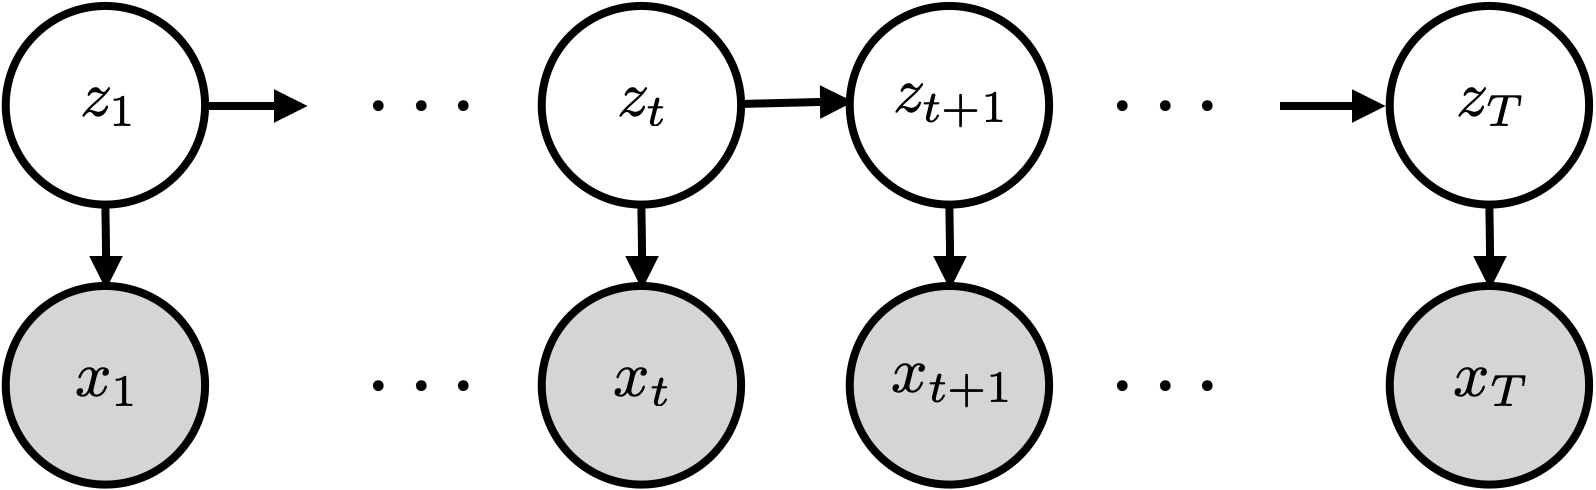
\includegraphics[width=0.7\textwidth]{11_hmms/hmm.png}    
    \end{center}
    
    This graphical model says that the joint distribution factors as,
    \begin{align}
        p(z_{1:T}, \mbx_{1:T}) &= p(z_1) \prod_{t=2}^T p(z_t \mid z_{t-1}) \prod_{t=1}^T p(\mbx_t \mid z_t).
    \end{align}
    
    We call this an HMM because $p(z_1) \prod_{t=2}^T p(z_t \mid z_{t-1})$ is a Markov chain.
\end{frame}    
    
\begin{frame}{State space models (SSMs)}
    Note that nothing above assumes that $z_t$ is a discrete random variable!
    
    HMM's are a special case of more general \textbf{state space models} with discrete states. 
    
    State space models assume the same graphical model but allow for arbitrary types of latent states. 
    
    For example, suppose that $\mbz_t \in \mathbb{R}^D$ are continuous valued latent states and that,
    \begin{align}
        p(\mbz_{1:T}) &= p(\mbz_1) \prod_{t=2}^T p(\mbz_t \mid \mbz_{t-1}) \\
        &= \cN(\mbz_1 \mid \mbb_1, \mbQ_1) \prod_{t=2}^T \cN(\mbz_t \mid \mbA \mbz_{t-1} + \mbb, \mbQ) 
    \end{align}
    This is called a Gaussian \textbf{linear dynamical system} (LDS). 
    \end{frame}
    
    \begin{frame}[t]{Stability of Gaussian linear dynamical systems}
        \textbf{Question: } What is the asymptotic mean of a Gaussian LDS, $\lim_{t \to \infty} \E[\mbz_t]$?
        
        \textbf{Question: } When is a Gaussian LDS stable? I.e. when is the asymptotic mean finite?
\end{frame}
    
\begin{frame}{Message passing in HMMs}
    
    In the HMM with discrete states, we showed how to compute posterior marginal distributions using message passing,
    \begin{align}
        p(z_t \mid \mbx_{1:T}) &\propto \sum_{z_1} \cdots \sum_{z_{t-1}} \sum_{z_{t+1}} \cdots \sum_{z_T} p(z_{1:T}, \mbx_{1:T}) \\
        &= \alpha_t(z_t) \, p(\mbx_t \mid z_t) \, \beta_t(z_t) 
    \end{align}
    where the \textit{forward and backward messages} are defined recursively
    \begin{align}
        \alpha_t(z_t) &= \sum_{z_{t-1}} p(z_t \mid z_{t-1}) \, p(\mbx_{t-1} \mid z_{t-1}) \, \alpha_{t-1}(z_{t-1}) \\
        \beta_t(z_t) &= \sum_{z_{t+1}} \, p(z_{t+1} \mid z_t) \, p(\mbx_{t+1} \mid z_{t+1}) \, \beta_{t+1}(z_{t+1})
    \end{align}
    The initial conditions are $\alpha_1(z_1) = p(z_1)$ and $\beta_{T}(z_T) = 1$.
        
\end{frame}
    
\begin{frame}{What do the forward messages tell us?}
    \label{slide:fwd_hmm}
    
    The forward messages are equivalent to,
    \begin{align}
        \alpha_t(z_t) &= \sum_{z_1} \cdots \sum_{z_{t-1}} p(z_{1:t}, \mbx_{1:t-1}) \\
        &p(z_t, \mbx_{1:t-1}).
    \end{align}
    The normalized message is the \textit{predictive distribution},
    \begin{align}
        \frac{\alpha_t(z_t)}{\sum_{z_t'} \alpha_t(z_t')} &= 
        \frac{p(z_t, \mbx_{1:t-1})}{\sum_{z_t'} p(z_t', \mbx_{1:t-1})} = \frac{p(z_t, \mbx_{1:t-1})}{p(\mbx_{1:t-1})} = p(z_t \mid \mbx_{1:t-1}),
    \end{align}
    The final normalizing constant yields the marginal likelihood, $\sum_{z_T} \alpha_T(z_T) = p(\mbx_{1:T})$.
    
    % Here, $z_t$ is a discrete random variable so we can think of the message as a vector,
    % \begin{align}
    %     \mbalpha_t &= [\alpha_{t1}, \ldots, \alpha_{tK}]^\top,
    % \end{align}
    % with  $\alpha_t(z_t)$ pulling out the $z_t$-th entry in this vector.
    
\end{frame}
    
\begin{frame}{Message passing in state space models}
    
    The same recursive algorithm applies (in theory) to any state space model with the same factorization, but the sums are replaced with integrals,
    \begin{align}
        p(\mbz_t \mid \mbx_{1:T}) &\propto \int \dif \mbz_1 \cdots \int \dif {\mbz_{t-1}} \int \dif{\mbz_{t+1}} \cdots \int \dif {\mbz_T} \,  p(\mbz_{1:T}, \mbx_{1:T}) \\
        &= \alpha_t(\mbz_t) \, p(\mbx_t \mid \mbz_t) \, \beta_t(\mbz_t) 
    \end{align}
    where the \textit{forward and backward messages} are defined recursively
    \begin{align}
        \alpha_t(\mbz_t) &= \int p(\mbz_t \mid \mbz_{t-1}) \, p(\mbx_{t-1} \mid \mbz_{t-1}) \, \alpha_{t-1}(\mbz_{t-1}) \dif {\mbz_{t-1}} \\
        \beta_t(\mbz_t) &= \int p(\mbz_{t+1} \mid \mbz_t) \, p(\mbx_{t+1} \mid \mbz_{t+1}) \, \beta_{t+1}(\mbz_{t+1}) \dif {\mbz_{t+1}} 
    \end{align}
    The initial conditions are $\alpha_1(\mbz_1) = p(\mbz_1)$ and $\beta_{T}(\mbz_T) \propto 1$.
        
\end{frame}
    
    % \begin{frame}[t]{Message passing in a linear dynamical system}
    % \textbf{Exercise:} Consider an LDS with Gaussian noise and assume that $p(\mbx_t \mid \mbz_t) = \cN(\mbx_t \mid \mbC \mbz_t + \mbd, \mbR)$. Derive the forward message $\alpha_t(\mbz_t)$ under the inductive hypothesis that $\alpha_{t-1}(\mbz_{t-1}) \propto \cN(\mbz_{t-1} \mid \mbmu_{t-1}, \mbSigma_{t-1})$.
    % \end{frame}
    
\begin{frame}[t]{Forward pass in a linear dynamical system}
    Consider an linear dynamical system (LDS) with Gaussian emissions,
    \begin{align}
        p(\mbx_{1:T}, \mbz_{1:T}) &= p(\mbz_1) \prod_{t=2}^T p(\mbz_t \mid \mbz_{t-1}) \\
        &= \cN(\mbz_1 \mid \mbb_1, \mbQ_1) \prod_{t=2}^T \cN(\mbz_t \mid \mbA \mbz_{t-1} + \mbb, \mbQ) \prod_{t=1}^ \cN(\mbx_t \mid \mbC \mbz_t + \mbd, \mbR)
    \end{align}
    
    Let's derive the forward message $\alpha_{t+1}(\mbz_{t+1})$. Assume $\alpha_{t}(\mbz_{t}) \propto \cN(\mbz_{t} \mid \mbmu_{t|t-1}, \mbSigma_{t|t-1})$.
    \begin{align}
        \alpha_{t+1}(\mbz_{t+1}) 
        &= \int p(\mbz_{t+1} \mid \mbz_{t}) \, p(\mbx_{t} \mid \mbz_{t}) \, \alpha_{t}(\mbz_{t}) \dif {\mbz_{t}} \\
        &= \int \cN(\mbz_{t+1} \mid \mbA \mbz_{t} + \mbb, \mbQ) \, \cN(\mbx_{t} \mid \mbC \mbz_{t} + \mbd, \mbR) \, \cN(\mbz_{t} \mid \mbmu_{t|t-1}, \mbSigma_{t|t-1}) \dif \mbz_{t}
    \end{align}
\end{frame}
    
\begin{frame}[t]{The update step}
    The first step is the \textbf{update step}, where we \textbf{condition on} the emission $\mbx_t$,
    
    \textbf{Exercise:} Expand the densities, collect terms, and complete the square to compute the mean $\mbmu_{t|t}$ and covariance $\mbSigma_{t|t}$ after the update step,
    \begin{align}
        \cN(\mbx_{t} \mid \mbC \mbz_{t} + \mbd, \mbR) \, \cN(\mbz_{t} \mid \mbmu_{t|t-1}, \mbSigma_{t|t-1}) 
        &\propto \cN(\mbz_t \mid \mbmu_{t|t}, \mbSigma_{t|t}).
    \end{align}
\end{frame}
    
    
\begin{frame}[t]{The update step II}
    Write the joint distribution,
    \begin{align}
        p(\mbz_t, \mbx_t \mid \mbx_{1:t-1}) 
        &= 
        \cN(\mbx_{t} \mid \mbC \mbz_{t} + \mbd, \mbR) \, \cN(\mbz_{t} \mid \mbmu_{t|t-1}, \mbSigma_{t|t-1}) \\
        &= 
        \cN \left(
        \begin{bmatrix}
        \mbz_t \\
        \mbx_t 
        \end{bmatrix}
        \, \bigg| \, 
        \begin{bmatrix}
        \mbmu_{t|t-1} \\
        \mbC \mbmu_{t|t-1} + \mbd
        \end{bmatrix},
        \begin{bmatrix}
        \mbSigma_{t|t-1} & \mbSigma_{t|t-1} \mbC^\top \\
        \mbC \mbSigma_{t|t-1} & \mbC \mbSigma_{t|t-1} \mbC^\top + \mbR
        \end{bmatrix}
        \right)
    \end{align}
    Since $(\mbz_t, \mbx_t)$ are jointly Gaussian, $\mbz_t$ must be conditionally Gaussian as well,
    \begin{align}
        p(\mbz_t \mid \mbx_{1:t}) &= \cN(\mbmu_{t|t}, \mbSigma_{t|t}).
    \end{align}
    \textbf{Exercise: } Now use the \textbf{Schur complement} from Week 1 to solve for $\mbmu_{t|t}$ and $\mbSigma_{t|t}$
    \end{frame}
    
    \begin{frame}[t]{The update step III}
    \textbf{Exercise: } Write $\mbmu_{t|t}$ and $\mbSigma_{t|t}$ in terms of the \textbf{Kalman gain},
    \begin{align}
        \mbK_t &= \mbSigma_{t|t-1} \mbC^\top (\mbC \mbSigma_{t|t-1} \mbC^\top + \mbR)^{-1}           
    \end{align}
    What is the Kalman gain doing?
    \end{frame}
    
    \begin{frame}[t]{The predict step}
    The predict step yields $p(\mbz_t \mid \mbx_{1:t}) = \cN(\mbz_t \mid \mbmu_{t|t}, \mbSigma_{t|t})$. To complete the forward pass, we need the \textbf{predict step},
    \begin{align}
        \alpha_{t+1}(\mbz_{t+1}) 
        &= \int p(\mbz_{t+1} \mid \mbz_{t}) \, p(\mbx_{t} \mid \mbz_{t}) \, \alpha_{t}(\mbz_{t}) \dif {\mbz_{t}} \\
        &= \int \cN(\mbz_{t+1} \mid \mbA \mbz_{t} + \mbb, \mbQ) \, \cN(\mbz_{t} \mid \mbmu_{t|t}, \mbSigma_{t|t}) \dif \mbz_{t} \\
        &= \cN(\mbz_{t+1} \mid \mbmu_{t+1|t}, \mbSigma_{t+1|t})
    \end{align}
    \textbf{Exercise: } Solve for the mean $\mbmu_{t+1|t}$ and covariance $\mbSigma_{t+1|t}$ after the predict step.
\end{frame}
    
\begin{frame}[t]{Completing the recursions}
    That wraps up the recursions! All that's left is the base case, which comes from the initial state distribution, 
    \begin{align}
        \mbmu_{1|0} = \mbb_1 \qquad \text{and} \quad \mbSigma_{1|0} = \mbQ_1.
    \end{align}
\end{frame}
    
\begin{frame}[t]{Computing the marginal likelihood}
    Like in the discrete HMM, we can compute the marginal likelihood along the forward pass.
    \begin{align}
    p(\mbx_{1:T}) 
    &= \prod_{t=1}^T p(\mbx_t \mid \mbx_{1:t-1}) \\
    &= \prod_{t=1}^T \int p(\mbx_t \mid \mbz_t) \, p(\mbz_t \mid \mbx_{1:t-1}) \dif \mbz_t \\
    &= \prod_{t=1}^T \int \cN(\mbx_t \mid \mbC \mbz_t + \mbd, \mbR) \, \cN(\mbz_t \mid \mbmu_{t|t-1}, \mbSigma_{t|t-1}) \dif \mbz_t 
    \end{align}
    \textbf{Exercise: } Obtain a closed form expression for the integrals.
\end{frame}
    
\begin{frame}{Computing the smoothing distributions}
    \begin{itemize}
        \item The forward pass gives us the filtering distributions $p(\mbz_t \mid \mbx_{1:t})$. How can we compute the smoothing distributions, $p(\mbz_t \mid \mbx_{1:\textcolor{red}{T}})$?
    
        \item In the discrete HMM we essentially ran the \textit{same algorithm in reverse} to get the backward messages, starting from $\beta_{T}(\mbz_T) \propto 1$.
    
        \item We can do the same sort of thing here, but it's a bit funky because we need to start with an improper Gaussian distribution $\beta_T(\mbz_T) \propto \cN(\mbzero, \infty \mbI)$.
        
        \item Instead, we'll derive an alternative way of computing the smoothing distributions.
    \end{itemize}
\end{frame}
    
\begin{frame}{Bayesian Smoothing}
        \textbf{Note:} $\mbz_t$ is conditionally independent of $\mbx_{t+1:T}$ given $\mbz_{t+1}$, so
        \begin{align}
            p(\mbz_t \mid \mbz_{t+1}, \mbx_{1:T}) 
            &= p(\mbz_t \mid \mbz_{t+1}, \mbx_{1:t}) \\
            &= \frac{p(\mbz_t, \mbz_{t+1} \mid \mbx_{1:t})}{p(\mbz_{t+1} \mid \mbx_{1:t})} \\
            &= \frac{p(\mbz_t \mid \mbx_{1:t}) \, p(\mbz_{t+1} \mid \mbz_t)}{p(\mbz_{t+1} \mid \mbx_{1:t})} 
        \end{align}
        \textbf{Question: } what rules did we apply in each of these steps?
\end{frame}
    
\begin{frame}{Bayesian Smoothing II}
    Now we can write the joint distribution as,
    \begin{align}
        p(\mbz_t, \mbz_{t+1} \mid \mbx_{1:T}) 
        &= p(\mbz_t \mid \mbz_{t+1} \mid \mbx_{1:T}) p(\mbz_{t+1} \mid \mbx_{1:T}) \\
        &= \frac{p(\mbz_t \mid \mbx_{1:t}) \, p(\mbz_{t+1} \mid \mbz_t) \,  p(\mbz_{t+1} \mid \mbx_{1:T})}{p(\mbz_{t+1} \mid \mbx_{1:t})}.
    \end{align}
    Marginalizing over $\mbz_{t+1}$ gives us,
    \begin{align}
        p(\mbz_t \mid \mbx_{1:T}) 
        &= p(\mbz_t \mid \mbx_{1:t}) \int \frac{p(\mbz_{t+1} \mid \mbz_t) \,  p(\mbz_{t+1} \mid \mbx_{1:T})}{p(\mbz_{t+1} \mid \mbx_{1:t})} \dif \mbz_{t+1}
    \end{align}
    \textbf{Question:} Can we compute each of these terms?
\end{frame}
    
\begin{frame}{The Rauch-Tung-Striebel Smoother, aka Kalman Smoother}
    These recursions apply to any Markovian state space model. For the special case of a Gaussian linear dynamical system, the smoothing distributions are again Gaussians,
    \begin{align}
        p(\mbz_t \mid \mbx_{1:T}) 
        &= \cN(\mbz_t \mid \mbmu_{t|T}, \mbSigma_{t|T}) 
    \end{align}
    where
    \begin{align}
        \mbmu_{t|T} &= \mbmu_{t|t} + \mbG_t (\mbmu_{t+1|T} - \mbmu_{t+1|t}) \\
        \mbSigma_{t|T} &= \mbSigma_{t|t} + \mbG_t (\mbSigma_{t+1|T} - \mbSigma_{t+1|t}) \mbG_t^\top \\
        \mbG_t &\triangleq \mbSigma_{t|t} \mbA^\top \mbSigma_{t+1|t}^{-1}.
    \end{align}
    This is called the \textbf{Rauch-Tung-Striebel (RTS) smoother} or the \textbf{Kalman smoother}.
\end{frame}


\begin{frame}[t,allowframebreaks]
    \frametitle{References}
    \bibliographystyle{unsrtnat}
    \bibliography{refs.bib}
\end{frame}

\end{document}
